% !TeX root = ../main.tex
% Add the above to each chapter to make compiling the PDF easier in some editors.

\chapter{TRACER: Automated Chatbot Exploration}\label{chapter:tracer}

In this chapter we present \ac{TRACER},
a tool that tries to fill the gaps that we have seen
during our State of the Art \autoref{sec:sota} review.
This tool's purpose is to address the black-box testing challenge mentioned
by iteratively discovering functionalities
to create a structured model.

The chapter will be structured with first
a high-level overview of the tool's two phase implementation \autoref{sec:overview}.
Then we will detail the exploration phase \autoref{sec:exploration},
followed by the refinement phase \autoref{sec:refinement}.

\section{Overview}\label{sec:overview}

\ac{TRACER} - \acl{TRACER} - the tool developed for this thesis,
whose source code can be found at \url{https://github.com/Chatbot-TRACER/TRACER},
is a tool that using the power of \acp{LLM}
is able to extract a model from a chatbot,
and then turn this model into a set of profiles
that can be used for the SENSEI user simulator
to test the chatbot.
An scheme of the proposed end-to-end testing
can be seen in \autoref{fig:approach}.

\begin{figure}[htpb]
  \centering
  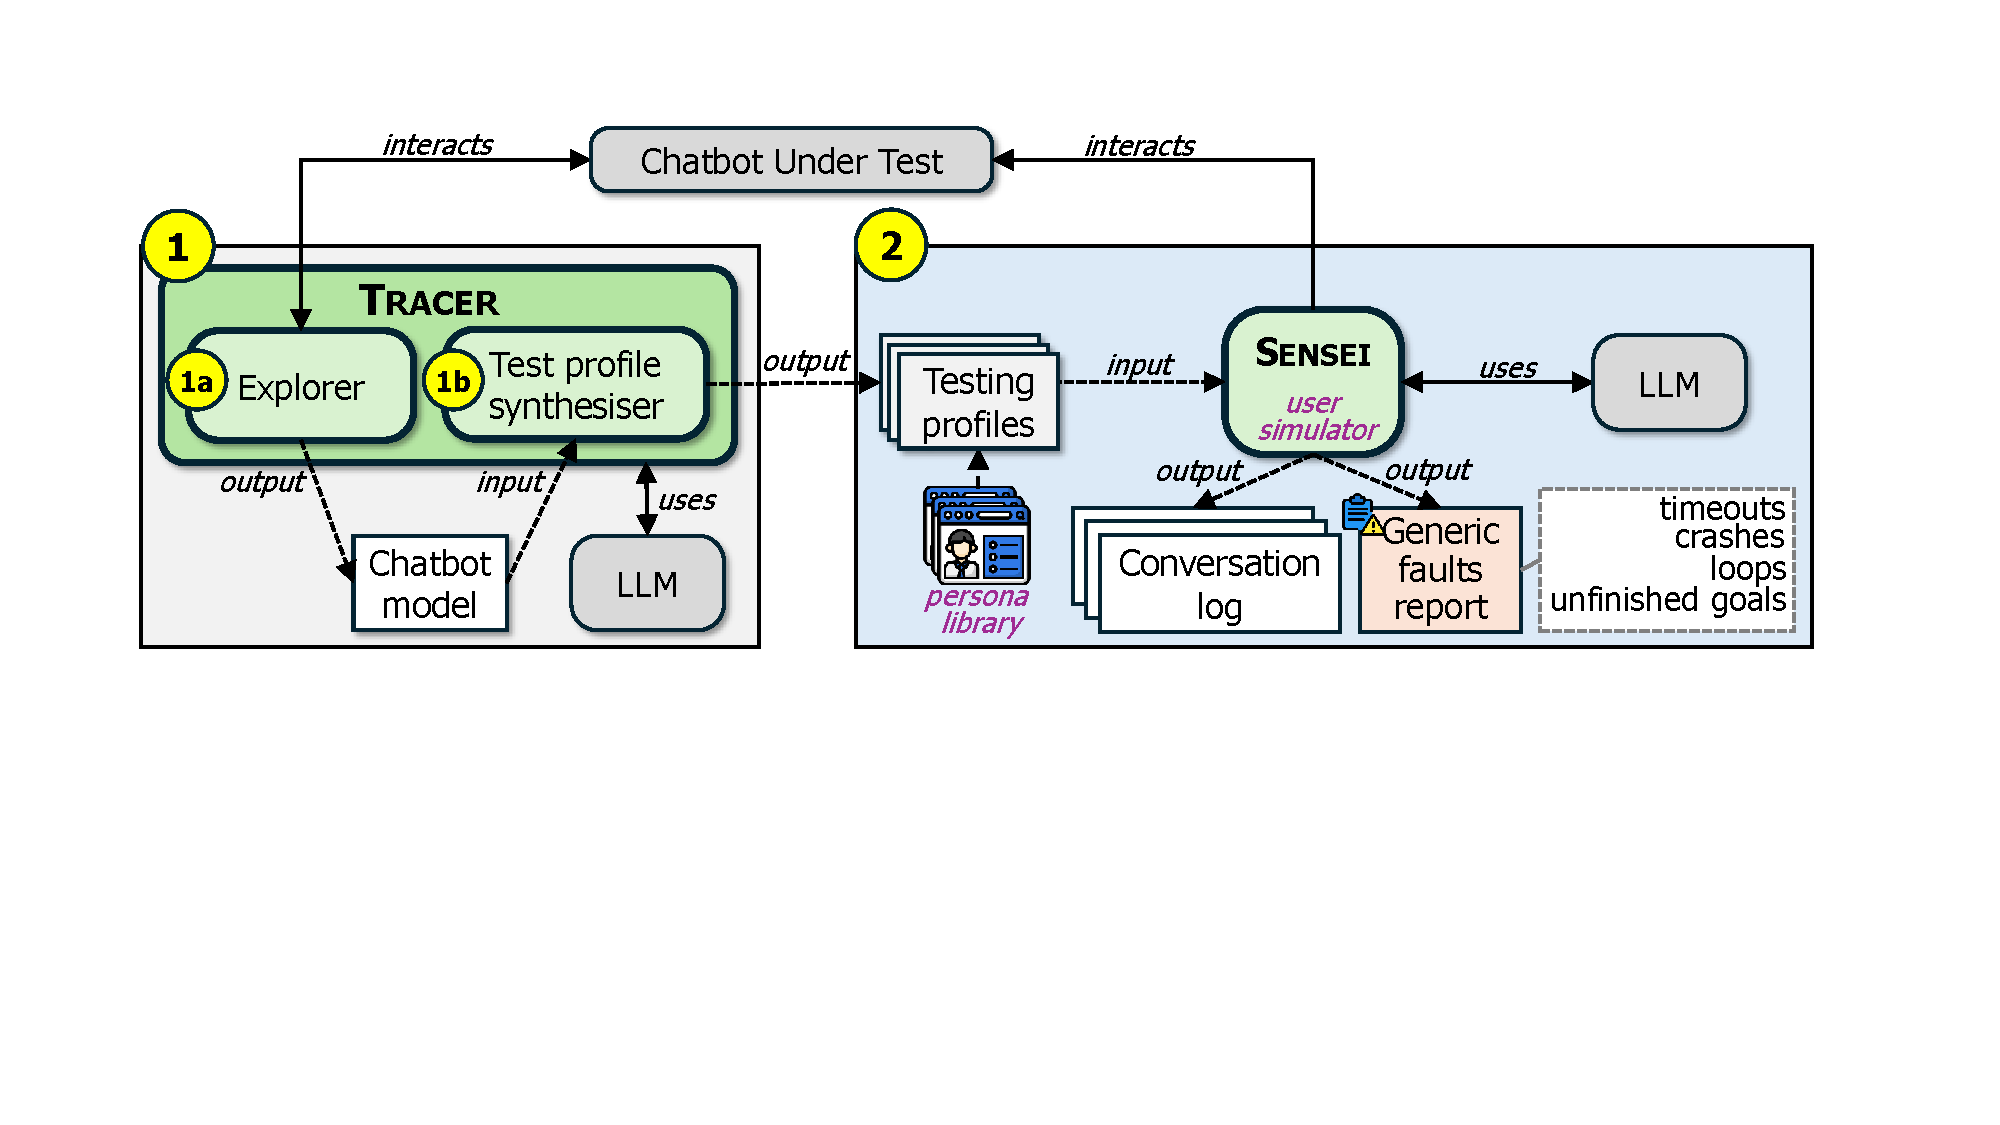
\includegraphics[width=\linewidth]{figures/approach.pdf}
  \caption{Scheme of our approach and its main components.
    (1a) Chatbot’s functionality explorer.
    (1b) Synthesiser of test conversation profiles.
    (2) User simulator.}
  \label{fig:approach}
\end{figure}


\begin{enumerate}
  \item \textbf{Exploration phase (1a):}
    an explorer agent interacts with the chatbot in multiple sessions
    and extracts a model of the chatbot
    The extracted model contains the following information:
    \begin{itemize}
      \item Language(s) that the chatbot understands.
      \item The chatbot's default fallback sentence (e.g., "I'm sorry, I can't undertand what you are saying.")
      \item The functionality graph.
    \end{itemize}

    The functionality graph, as its name implies,
    is a graph, precisely, a \ac{DAG}
    that mimics the workflow of the chatbot.
    Its nodes are functionality nodes,
    an object that contains all the information regarding a functionality
    (will be explained further in 
    \autoref{sec:exploration}).

  \item \textbf{Refinement phase (1b):}
    in this pase the extracted model will be refined,
    similar functionalities will be merged,
    and order of the nodes in the \ac{DAG} will be revised
    so that it matches the chatbot's workflow.
    Once we have this final model,
    the user profiles for SENSEI will be created based on this model.
    The profiles will have goals, context, roles and outputs
    that will match what is found on the model.

  \item \textbf{User simulator (2):}
    Once the model and user profiles have been created,
    we use the profiles within SENSEI, the user simulator.
    During the simulation,
    we can find crashes, conversation loops, timeouts,
    or unfinished goals (i.e., tasks that the user profile had
    but was not able to achieve, like ordering a pizza).
    It is important to note that
    although SENSEI is an important part in this testing process
    it has not been developed in this work.
\end{enumerate}



\section{Exploration Phase}\label{sec:exploration}

\section{Refinement Phase}\label{sec:refinement}


